% The comment below tells Rubber to compile the .dot files.
%
% rubber: module graphics
% rubber: rules rules.ini

\documentclass{beamer}

\usetheme{default}

\usepackage{helvet}
\usecolortheme{seagull}         % white on black

\usepackage[utf8]{inputenc}
\PassOptionsToPackage{hyphens}{url}\usepackage{hyperref,xspace,multicol}
\usepackage[absolute,overlay]{textpos}
\usepackage{tikz}
\usetikzlibrary{arrows,shapes,trees,shadows,positioning}
\usepackage{fancyvrb}           % for \Verb

% Remember the position of every picture.
\tikzstyle{every picture}+=[remember picture]

\tikzset{onslide/.code args={<#1>#2}{%
  \only<#1>{\pgfkeysalso{#2}} % \pgfkeysalso doesn't change the path
}}

% Colors.
\definecolor{guixred1}{RGB}{226,0,38}  % red P
\definecolor{guixorange1}{RGB}{243,154,38}  % guixorange P
\definecolor{guixyellow}{RGB}{254,205,27}  % guixyellow P
\definecolor{guixred2}{RGB}{230,68,57}  % red S
\definecolor{guixorange2}{RGB}{236,117,40}  % guixorange S
\definecolor{guixtaupe}{RGB}{134,113,127} % guixtaupe S
\definecolor{guixgrey}{RGB}{91,94,111} % guixgrey S
\definecolor{guixblue1}{RGB}{38,109,131} % guixblue S
\definecolor{guixblue2}{RGB}{10,50,80} % guixblue S
\definecolor{guixgreen1}{RGB}{133,146,66} % guixgreen S
\definecolor{guixgreen2}{RGB}{157,193,7} % guixgreen S

\setbeamerfont{title}{size=\huge}
\setbeamerfont{frametitle}{size=\huge}

% White-on-black color theme.
\setbeamercolor{structure}{fg=guixorange1,bg=black}
\setbeamercolor{title}{fg=white,bg=black}
\setbeamercolor{date}{fg=guixorange1,bg=black}
\setbeamercolor{frametitle}{fg=white,bg=black}
\setbeamercolor{titlelike}{fg=white,bg=black}
\setbeamercolor{normal text}{fg=white,bg=black}
\setbeamercolor{alerted text}{fg=guixyellow,bg=black}
\setbeamercolor{section in toc}{fg=white,bg=black}
\setbeamercolor{section in toc shaded}{fg=white,bg=black}
\setbeamercolor{subsection in toc}{fg=guixorange1,bg=black}
\setbeamercolor{subsection in toc shaded}{fg=white,bg=black}
\setbeamercolor{subsubsection in toc}{fg=guixorange1,bg=black}
\setbeamercolor{subsubsection in toc shaded}{fg=white,bg=black}
\setbeamercolor{frametitle in toc}{fg=white,bg=black}
\setbeamercolor{local structure}{fg=guixorange1,bg=black}

\newcommand{\highlight}[1]{\alert{\textbf{#1}}}

\title{Reproducible and User-Controlled Package Management in HPC with GNU Guix}

\author{Ludovic Courtès (\texttt{ludovic.courtes@inria.fr})
  \\Ricardo Wurmus (\texttt{ricardo.wurmus@mdc-berlin.de})}
\date{\small{Workshop on Reproducibility in Parallel Computing
    (RepPar)\\25 August 2015}}

\setbeamertemplate{navigation symbols}{} % remove the navigation bar

\AtBeginSection[]{
  \begin{frame}
    \frametitle{}
    \tableofcontents[currentsection]
  \end{frame} 
}


\begin{document}

\maketitle


% HPC system administration has to satisfy two seemingly
% contradictory demands: on one hand administrators seek stability,
% which leads to a conservative approach to software management, and
% on the other hand users demand recent tool chains and huge
% scientific software stacks.  In addition, users often need
% different versions and different variants of a given software
% package.

% To satisfy both, support teams build and install tool
% chains, libraries, and scientific software packages
% manually---multiple variants thereof---and make them available
% via ``environment modules''.

% However, HPC system users have no guarantee that they will be able
% to reproduce results at a later point in time, even on the same
% system---software may have been upgraded, removed, or recompiled
% under their feet, and they have little hope of being able to
% reproduce the same software environment elsewhere.

\begin{frame}{``Reproducibility''?}
  % Let us first define what the term "reproducibility" means when
  % applied to software and software environments in the context of
  % this talk.

  \Large{
    \begin{enumerate}
      % The most obvious and yet most elusive is reproducible software
      % builds, i.e. translating source code into bit-identical
      % binaries, across independent builds.
    \item<2-> \textbf{bit-reproducible} builds

      % Another is keeping a software *environment* constant,
      % i.e. reproducing the environment for one user on the same
      % machine across time.
    \item<3-> \textbf{isolating} a software environment from changes

      \only<4> {
        \begin{tikzpicture}[overlay]
          \node [at=(current page.center), inner sep=0mm]{
            \includegraphics[width=\textwidth]{images/isolation-1}
          };
        \end{tikzpicture}
      }

      \only<5> {
        \begin{tikzpicture}[overlay]
          \node [at=(current page.center), inner sep=0mm]{
            \includegraphics[width=\textwidth]{images/isolation-2}
          };
        \end{tikzpicture}
      }


      % And lastly, as an extension to the previous case, reproducing
      % an environment on a different machine and at a different point
      % in time, i.e. sharing an environment with others.
    \item<6-> \textbf{sharing} environments with others
      \only<7> {
        \begin{tikzpicture}[overlay]
          \node [at=(current page.center), inner sep=0mm]{
            \includegraphics[width=\textwidth]{images/isolation-2}
          };
        \end{tikzpicture}
      }

      \only<8> {
        \begin{tikzpicture}[overlay]
          \node [at=(current page.center), inner sep=0mm]{
            \includegraphics[width=\textwidth]{images/sharing}
          };
        \end{tikzpicture}
      }

    \end{enumerate}
  }
\end{frame}

\begin{frame}{Beyond Reproducibility}
  % To make science reproducible, it is not enough to just
  % "shrink-wrap" environments.  A necessary requirement to verifying
  % methods and results is the ability to experiment with the system.
  % The steps *after* reproducing an environment are just as
  % important as getting the environment set up in the first place.

  \Large{
    \begin{itemize}
      % The user (and nobody else) needs to have control over changes
      % the environment.  It should be easy to safely revert
      % changes and continue exploration with previous versions, to
      % make exploration cheap.
    \item<2-> \textbf{user-controlled upgrades} and roll-backs
      \only<3> {
        \begin{tikzpicture}[overlay]
          \node [at=(current page.center), inner sep=0mm]{
            \includegraphics[width=\textwidth]{images/isolation-2}
          };
        \end{tikzpicture}
      }

      \only<4> {
        \begin{tikzpicture}[overlay]
          \node [at=(current page.center), inner sep=0mm]{
            \includegraphics[width=\textwidth]{images/upgrades}
          };
        \end{tikzpicture}
      }


      % Changing *specific* parts of the software stack (e.g. a
      % dependent library, or the toolchain) must be possible to see
      % what impact they have on the result.
    \item<5-> change \textbf{specific parts} of the software stack
      \only<6> {
        \begin{tikzpicture}[overlay]
          \node [at=(current page.center), inner sep=0mm]{
            \includegraphics[width=\textwidth]{images/upgrades}
          };
        \end{tikzpicture}
      }

      \only<7> {
        \begin{tikzpicture}[overlay]
          \node [at=(current page.center), inner sep=0mm]{
            \includegraphics[width=\textwidth]{images/specific-changes}
          };
        \end{tikzpicture}
      }

      % Users should not be limited by an opaque system that cannot be
      % inspected.  It is hard to draw any scientific conclusion from
      % an experiment that relies on black boxes.
    \item<8-> \textbf{hackability}: no black boxes
    \end{itemize}
  }
\end{frame}


\begin{frame}{VMs and Docker}
  % A popular response to problems relating to deploying software
  % environments is full system virtualization or, more recently,
  % a system that makes use of containers, such as Docker.

  % This means you develop in a VM and once you're satisfied publish
  % the image; or you write and publish a Dockerfile that prescibes
  % how a base image is to be modified to reach the desired state.

  \Large{
  \begin{columns}
    \begin{column}[t]<2->{0.5\textwidth}
      Pros:
      \begin{itemize}
        % It's bit-reproducible in the sense that you essentially
        % publish the bits.
      \item ``bit-reproducible''

        % Virtualization is wide-spread and is "proven technology" with
        % few surprises, making it simple for anyone to reuse an image.
      \item reproducible anywhere by anyone
      \end{itemize}
    \end{column}

    \begin{column}[t]<3->{0.5\textwidth}
      Problems:
      \begin{itemize}
        % VMs are heavyweight, which means they are unsuited for HPC.
        % * hardware support + KVM + in-kernel page deduplication help, but still
      \item VMs are heavyweight

        % VM images are completely opaque, binary artifacts: how can I
        % reproduce them?
        % Likewise, Dockerfiles describe steps to modify an opaque base
        % image.  How was the base image produced?  Do the binary
        % packages of the base system really correspond
        % to the source they claim to come from?

        % In both cases, inspection is difficult: we're given a pizza,
        % but not its recipe.
        % * {image of frozen pizza}
        % * {image of a very detailed recipe}
      \item binary images are opaque

        % The full system image is standalone by definition.  There is
        % no way to use the software embedded in the image *alongside*
        % other software packages I may need.

        % For example, there is no way to use, say, the library that's
        % inside the system image as-is in my own software system.

        % This encourages bad habits: modifying the image
        % state by building additional software in an ad-hoc
        % manner---we're giving up on isolation and good system
        % administration techniques.
      \item not composable
      \end{itemize}
    \end{column}
  \end{columns}
  }
\end{frame}

%% \section{Functional Package Management}

\setbeamercolor{normal text}{bg=guixblue2}
\begin{frame}[plain]
  \center{\Huge{\textbf{Functional Package Management}}}
\end{frame}
\setbeamercolor{normal text}{fg=white,bg=black}

\begin{frame}{Functional Package Management}
  \Large{
    Regarding the build \& installation process
    of a package as a \highlight{pure function}.
  }
\end{frame}

\begin{frame}[plain]
  \Large{
    $\texttt{openmpi} = f(\texttt{hwloc}, \texttt{gcc}, \texttt{make},\texttt{coreutils})$
    
    \uncover<2->{$\texttt{hwloc} = g(\texttt{pciaccess}, \texttt{gcc}, \texttt{make}, \texttt{coreutils})$}

    \uncover<3->{$\texttt{gcc} = h(\texttt{make}, \texttt{coreutils}, \texttt{gcc}_0)$}
    
    \uncover<3->{\textrm{...}}
  }

  \uncover<1>{\large{where $f =$ \texttt{./configure \&\& make \&\& make install}}}

  \begin{tikzpicture}[overlay]
    \node<4->[fill=guixorange1, text=black, text opacity=1, opacity=.7,
          rounded corners=2mm, inner sep=5mm] at (5, 1) {
            \textbf{\Large{the complete DAG is captured}}
          };
  \end{tikzpicture}
\end{frame}

\begin{frame}{References}
  \Large{
    \begin{itemize}
    %% \item<3-> \textit{Caching Function Calls Using Precise Dependencies}
    %%   (``Vesta''), Heydon et al., 2000
    \item \textit{A Safe and Policy-Free System for Software Deployment}
      (``Nix''), Dolstra et al., 2003
    \item \textit{Functional Package Management with Guix}, Courtès,
      2013
    \end{itemize}
  }
\end{frame}

\begin{frame}{Thesis}

  \Large{
    \begin{enumerate}
    \item functional package management (FPM) \textbf{empowers cluster
      users}
    \item FPM is a solid foundation for \textbf{reproducible software
      deployment}
    \item \textbf{beyond reproducibility}: Guix is programmable, supports
      experimentation
      % You get the ``source of the software environment''.
    \end{enumerate}
  }
\end{frame}

\begin{frame}[fragile]
  \frametitle{From the Architecture of Nix...}
  \framesubtitle{\url{http://nixos.org/nix/}}

  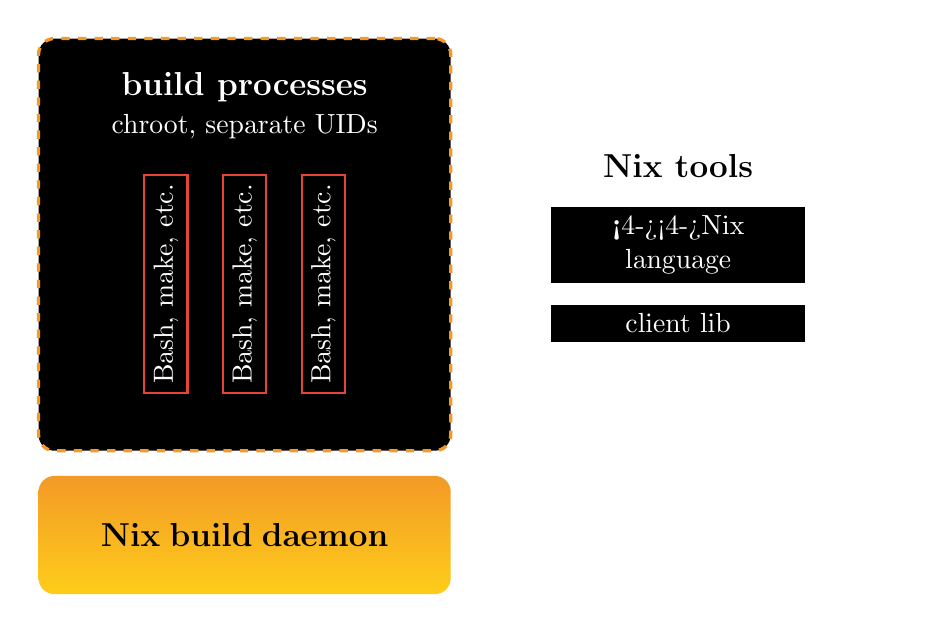
\begin{tikzpicture}[tools/.style = {
                        text width=35mm, minimum height=4cm,
                        text centered,
                        rounded corners=2mm,
                        fill=white, text=black
                      },
                      tool/.style = {
                        fill=black, text=white, text width=3cm,
                        text centered
                      },
                      daemon/.style = {
                        rectangle, text width=50mm, text centered,
                        rounded corners=2mm, minimum height=15mm,
                        top color=guixorange1,
                        bottom color=guixyellow,
                        text=black
                      },
                      builders/.style = {
                        draw=guixorange1, very thick, dashed,
                        fill=black, text=white, text width=5cm,
                        rounded corners=2mm,
                      },
                      builder/.style = {
                        draw=guixred2, thick, rectangle,
                        fill=black, text=white,
                        rotate=90
                      }]
    \matrix[row sep=3mm, column sep=1cm] {
      \node(builders)[builders, text height=5cm]{}
          node[fill=black, text=white] at (0, 2) {\large{\textbf{build processes}}}
          node[fill=black, text=white] at (0, 1.5) {chroot, separate UIDs}
          node[builder, onslide=<1-2>{black}] at (-1,-0.5) {Bash, make, etc.}
          node[builder, onslide=<1-2>{black}] at ( 0,-0.5) {Bash, make, etc.}
          node[builder, onslide=<1-2>{black}] at ( 1,-0.5) {Bash, make, etc.}; &
      \node[tools]{}
          node[fill=white, text=black] at (0, 1) {\large{\textbf{Nix tools}}}
          node[tool] at (0, 0) {\textbf<4->{\alert<4->{Nix language}}}
          node(client)[tool] at (0, -1) {client lib};
      \\

      \node(daemon)[daemon]{\large{\textbf{Nix build daemon}}}; &
      &
      \\
    };
  \end{tikzpicture}

  \begin{tikzpicture}[overlay]
    \path[very thick, draw=guixorange1]<2->
      (client.south) edge [out=-90, in=0, ->] node[below, sloped]{RPCs} (daemon.east);
    \path[->, very thick, draw=guixorange1]<3->
      (daemon) edge (builders);
  \end{tikzpicture}
\end{frame}

\begin{frame}[fragile]
  \frametitle{... to the Architecture of Guix}
  \framesubtitle{\url{http://gnu.org/s/guix/}}

  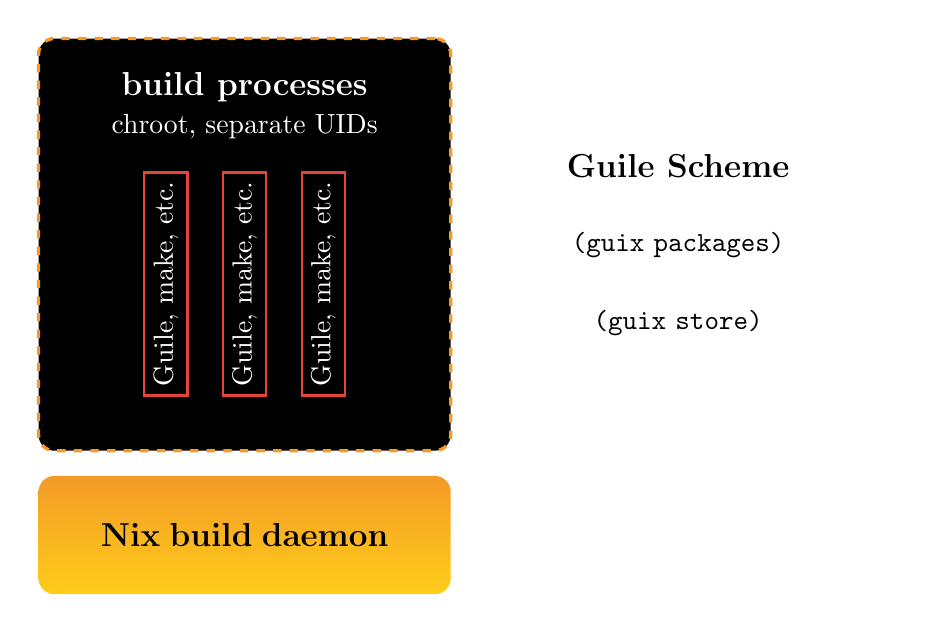
\begin{tikzpicture}[tools/.style = {
                        text width=35mm, minimum height=4cm,
                        text centered,
                        rounded corners=2mm,
                        fill=white, text=black
                      },
                      tool/.style = {
                        fill=white, text=black, text width=3cm,
                        text centered
                      },
                      daemon/.style = {
                        rectangle, text width=50mm, text centered,
                        rounded corners=2mm, minimum height=15mm,
                        top color=guixorange1,
                        bottom color=guixyellow,
                        text=black
                      },
                      builders/.style = {
                        draw=guixorange1, very thick, dashed,
                        fill=black, text=white, text width=5cm,
                        rounded corners=2mm,
                      },
                      builder/.style = {
                        draw=guixred2, thick, rectangle,
                        fill=black, text=white,
                        rotate=90
                      }]
    \matrix[row sep=3mm, column sep=1cm] {
      \node(builders)[builders, text height=5cm]{}
          node[fill=black, text=white] at (0, 2) {\large{\textbf{build processes}}}
          node[fill=black, text=white] at (0, 1.5) {chroot, separate UIDs}
          node[builder] at (-1,-0.5) {\alert{Guile}, make, etc.}
          node[builder] at ( 0,-0.5) {\alert{Guile}, make, etc.}
          node[builder] at ( 1,-0.5) {\alert{Guile}, make, etc.}; &
      \node[tools]{}
          node[fill=white, text=black] at (0, 1) {\large{\textbf{Guile Scheme}}}
          node[tool] at (0, 0) {\texttt{(guix packages)}}
          node(client)[tool] at (0, -1) {\texttt{(guix store)}};
      \\

      \node(daemon)[daemon]{\large{\textbf{Nix build daemon}}}; &
      &
      \\
    };
  \end{tikzpicture}

  \begin{tikzpicture}[overlay]
    \path[very thick, draw=guixorange1]
      (client.south) edge [out=-90, in=0, ->] node[below, sloped]{RPCs} (daemon.east);
    \path[->, very thick, draw=guixorange1]
      (daemon) edge (builders);
  \end{tikzpicture}
\end{frame}

\begin{frame}[fragile]
  \frametitle{Why Guix?}
  \framesubtitle{[Courtès 2013]}

  \Large{
    \begin{enumerate}
    \item{Scheme is a ``programmable programming language''
      $\rightarrow$ \alert{tailored EDSLs}}
    \item \alert{general-purpose language} with compiler, debugger,
      libraries, etc.
    \item \alert{a single language} $\rightarrow$ more code reuse,
      unified environment
    \item \highlight{complete package programming interface}
    \end{enumerate}
  }
\end{frame}

\begin{frame}[fragile]
  \frametitle{Bit-Reproducible Builds$^*$}
  \framesubtitle{$^*$ almost!}

  \begin{semiverbatim}
\$ guix build petsc
\uncover<2->{/gnu/store/\tikz[baseline]{\node[anchor=base](nixhash){\alert<2>{h2g4sf72\textrm{...}}};}-petsc-3.6.0}

\uncover<3->{\$ \alert<3>{guix gc --references /gnu/store/\textrm{...}-petsc-3.6.0}
/gnu/store/\textrm{...}-openmpi-1.8.5
/gnu/store/\textrm{...}-gfortran-4.9.3-lib
/gnu/store/\textrm{...}-superlu-4.3
/gnu/store/\textrm{...}-lapack-3.5.0
/gnu/store/\textrm{...}-glibc-2.21
\textrm{...}}
  \end{semiverbatim}

  \begin{tikzpicture}[overlay]
    \node<1>(labelnixhash) [fill=white, text=black] at (current page.center) {%
      \Large{\textbf{isolated build}: chroot, separate name spaces, etc.}
    };

    \node<2>(labelnixhash) [fill=white, text=black] at (4cm, 2cm) {%
      hash of \textbf{all} the dependencies};
    \path[->]<2>(labelnixhash.north) edge [bend left, in=180, out=-45] (nixhash.south);

    \draw<4-> (-10pt, 105pt) [very thick, color=guixorange2, rounded corners=8pt]
      arc (10:-50:-50pt and 110pt);
    \node<4->[fill=white, text=black, text opacity=1, opacity=.7,
          rounded corners=2mm, inner sep=5mm]
      at (7, 2) {\textbf{\Large{(nearly) bit-identical for everyone}}};
    %% \node<5>[fill=white, text=black, text opacity=1, opacity=.7,
    %%       rounded corners=1mm, inner sep=3mm]
    %%   at (8, 1) {\url{http://reproducible.debian.net}};
  \end{tikzpicture}

\end{frame}

\begin{frame}[fragile]
  \frametitle{Reproducible Environments}

  \Large{
    \begin{itemize}
    \item \textbf{per-user ``profiles''}
    \item \textbf{non-interference} among users/profiles
    \item \textbf{transactional upgrades \& rollbacks}
    \end{itemize}
  }
\end{frame}

\begin{frame}[fragile]
  \frametitle{Reproducible Environments}

  \begin{semiverbatim}
\$ guix package -i gcc-toolchain coreutils sed grep
\textrm{...}

\$ eval `guix package --search-paths`
\textrm{...}

\$ guix package --manifest=my-software.scm
\textrm{...}

\$ guix environment petsc
\textrm{...}

\$ guix environment --ad-hoc python-ipython python-numpy \\
    -E ipython
\textrm{...}
  \end{semiverbatim}

  \begin{tikzpicture}[overlay]
    \node[rounded corners=4, text centered,
          fill=guixorange1, text width=3cm,
          inner sep=3mm, rotate=5, opacity=.75, text opacity=1,
          drop shadow={opacity=0.5}] at (5, 4) {
            \textbf{\large{demo}}
          };
  \end{tikzpicture}
\end{frame}

\begin{frame}
  \frametitle{Experience at the\\Max Delbrück Center, Berlin}

  \large{
  \begin{itemize}
    \item \textbf{Guix deployed on two clusters} ($\approx$250 nodes) + workstations
    \item used by \textbf{bioinformatics} researchers
    \item \textbf{50+ bioinfo packages} in use (C/C++, Python,
      etc.)
    \item replaces CentOS packages + sysadmin-managed software
    \item<2-> \highlight{advantages}: more user control, better resource
      usage, ...
  \end{itemize}
  }
\end{frame}

\setbeamercolor{normal text}{bg=guixblue2}
\begin{frame}[plain]
  \center{\Huge{\textbf{Beyond Reproducibility:\\
        Supporting Experimentation}}}
\end{frame}
\setbeamercolor{normal text}{fg=white,bg=black}

\begin{frame}[fragile]
  \frametitle{Fiddling with the HPC Stack}
  \framesubtitle{Example from Inria}

  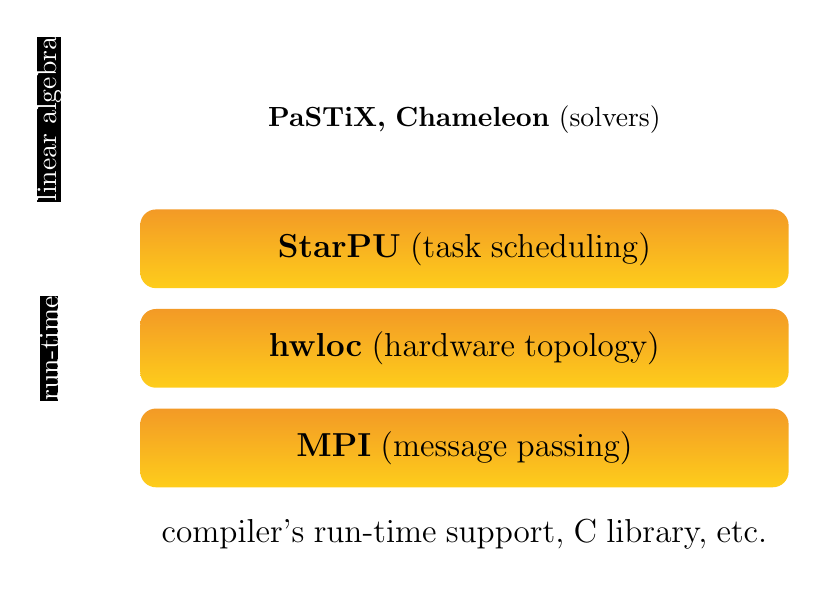
\begin{tikzpicture}[algebra/.style = {
                        text width=8cm, text centered,
                        rounded corners=2mm,
                        minimum height=2cm,
                        fill=white, text=black
                      },
                      runtime/.style = {
                        text width=8cm, text centered,
                        rounded corners=2mm,
                        minimum height=1cm,
                        top color=guixorange1,
                        bottom color=guixyellow,
                        text=black
                      },
                      system/.style = {
                        text width=8cm, text centered,
                        rounded corners=2mm,
                        fill=white, text=black,
                        minimum height=1cm
                      },
                      legend/.style = {
                        fill=black, text=white, rotate=90,
                        inner sep=0mm
                      }]
    \matrix[row sep=1mm, column sep=1cm] {
      \node[legend]{linear algebra}; &
      \node[algebra]{\textbf{PaSTiX, Chameleon} (solvers)};
      \\

      &
      \node[runtime]{\large{\textbf{StarPU}} (task scheduling)};
      \\

      \node[legend]{run-time}; &
      \node[runtime]{\large{\textbf{hwloc}} (hardware topology)};
      \\

      &
      \node[runtime]{\large{\textbf{MPI}} (message passing)};
      \\

      &
      \node[system]{\large{compiler's run-time support, C~library,
          etc.}}; \\ };
  \end{tikzpicture}
\end{frame}

\begin{frame}{Requirements for an\\Experimentation-Capable System}

  \Large{
    \begin{enumerate}
    \item customize + non-ambiguously \highlight{specify package DAG}
    \item reliably reproduce \highlight{variants of the DAG}
    \end{enumerate}
  }
\end{frame}

\begin{frame}[fragile]
  \begin{semiverbatim}
\small{
(define starpu
  (\alert{package}
    (name "starpu")
    (version "1.1.4")
    (source (origin
             (method url-fetch)
             (uri "http://\textrm{...}")
             (sha256 (base32 "0zmkw\textrm{...}"))))
    (\alert{build-system} \tikz[baseline]{\node[anchor=base](gbs){gnu-build-system};})
    (native-inputs `(("pkg-config" ,pkg-config)))
    (\tikz[baseline]{\node[anchor=base](deps){inputs};} `(("fftw" ,fftw)
              ("hwloc" ,\tikz[baseline]{\node[anchor=base](var){hwloc};})))
    (home-page "http://starpu.gforge.inria.fr/")
    (synopsis "Run-time system for heterogeneous computing")
    (description "Blah...")
    (license lgpl2.1+)))
}
  \end{semiverbatim}

  \begin{textblock}{5}(11, 12)
    \tikz{\node<2>(labeldeps)[fill=white, text=black]{dependencies};}
  \end{textblock}

  %% \begin{textblock}{5}(9, 9)
  %%   \tikz{\node<3>(labelvar)[fill=white, text=black]{reference to a
  %%       variable};}
  %% \end{textblock}

  \begin{textblock}{5}(3, 5)
    \tikz{\node<3>(labelgbs)[fill=white, text=black]{\texttt{./configure
        \&\& make install}...};}
  \end{textblock}

  \begin{textblock}{5}(8, 9)
    \tikz{\node<3>(labelgbsdeps)[fill=white, text=black]{depends on
        \texttt{gcc}, \texttt{make}, \texttt{bash}, etc.};}
  \end{textblock}

  \begin{tikzpicture}[overlay]
    \path[->, fill=white, thick]<2>(labeldeps) edge (deps);
    %% \path[->, fill=white, thick]<3>(labelvar) edge (var);
    \path[->, fill=white, thick]<3>(labelgbs) edge (gbs);
    \path[->, fill=white, thick]<3>(labelgbsdeps) edge (gbs);
  \end{tikzpicture}
\end{frame}

\begin{frame}[plain]
  \frametitle{DAG of Package Objects}

  \begin{tikzpicture}[overlay]
    \node [at=(current page.center), inner sep=0mm]{
      \includegraphics[width=1.3\textwidth]{starpu-package-dag}
    };
    \node (command) [at=(current page.south east), anchor=south east, inner sep=5mm]{
      \texttt{guix graph --type=package starpu}
    };
    \node [at=(current page.south west), anchor=south west, inner sep=5mm]{
      \Large{\highlight{10 nodes}}
    };
    \node<2->[fill=guixorange1, text=black, text opacity=1, opacity=.7,
      rounded corners=2mm, inner sep=5mm, at=(current page.center)] {
      \textbf{\Large{Where are GCC, libc, etc.?}}
    };
  \end{tikzpicture}
\end{frame}

\begin{frame}[plain]
  \frametitle{Same DAG, including implicit inputs}

  \begin{tikzpicture}[overlay]
    \node [at=(current page.center), inner sep=0mm]{
      \includegraphics[width=1.2\textwidth]{starpu-emerged-dag}
    };
    \node [at=(current page.south west), anchor=south west, inner sep=5mm]{
      \Large{\highlight{29 nodes}}
    };
    \node [at=(current page.south east), anchor=south east, inner sep=5mm]{
      \texttt{guix graph --type=bag-emerged starpu}
    };
    \node<2->[fill=guixorange1, text=black, text opacity=1, opacity=.7,
      rounded corners=2mm, inner sep=5mm, at=(current page.center)] {
      \textbf{\Large{What about the compiler's compiler, etc.?}}
    };
  \end{tikzpicture}
\end{frame}

\begin{frame}[plain]
  \frametitle{Full DAG, including bootstrap}

  \begin{tikzpicture}[overlay]
    \node [at=(current page.center), inner sep=0mm]{
      %\includegraphics[width=0.01\textwidth]{starpu-full-dag}
      \large{(too big)}
    };
    \node [at=(current page.south west), anchor=south west, inner sep=5mm]{
      \Large{\highlight{321 nodes}}
    };
    \node [at=(current page.south east), anchor=south east, inner sep=5mm]{
      \texttt{guix graph --type=bag starpu}
    };
  \end{tikzpicture}
\end{frame}

\begin{frame}[fragile]
  \frametitle{Defining Package Variants}

  \begin{semiverbatim}
\small{
(define starpu-1.2rc              ;release candidate
  (package (\alert{inherit} starpu)
    (version "1.2.0rc2")
    (source (origin
             (method url-fetch)
             (uri (string-append "http://\textrm{...}/"
                                 "starpu-" version ".tar.gz"))
             (sha256 (base32 "0qgb6y\textrm{...}"))))))
}
  \end{semiverbatim}
\end{frame}

\begin{frame}[fragile]
  \frametitle{Defining Package Variants}
  
  \begin{semiverbatim}
\small{
(define starpu-with-simgrid
  (package (\alert{inherit} starpu)
    (name "starpu-with-simgrid")

    ;; Add SimGrid, an optional dependency.
    (inputs `(("simgrid" ,simgrid)
              ,@(package-inputs starpu)))))
}
  \end{semiverbatim}
\end{frame}

\begin{frame}[fragile]
  \frametitle{Package Functions}

  \begin{semiverbatim}
\small{
  (define (\alert{make-chameleon} \tikz[baseline]{\node(formal)[anchor=base]{\alert<1>{starpu}};})
     ;; Return the Chameleon solver linked against
     ;; this particular variant of StarPU.
     (\alert{package}
       ;; \textrm{...}
       (inputs `(("starpu" ,\tikz[baseline]{\node(use)[anchor=base]{\alert<1>{starpu}};})
                 ("blas" ,atlas)
                 ("lapack" ,lapack)
                 ("gfortran" ,gfortran-4.8)
                 ("python" ,python-2)))))
\uncover<2->{
   (define chameleon
     (\alert{make-chameleon} starpu))
   (define chameleon/starpu-simgrid
     (\alert{make-chameleon} starpu-with-simgrid))
}
}
  \end{semiverbatim}

  \begin{tikzpicture}[overlay]
    \path[<->, fill=white, thick]<1>(formal) edge (use);
  \end{tikzpicture}
\end{frame}

%%%%%%%%%%%%%%%%%%%%%%%%%%%%%%%%%%%%%%%%%%%%%%%%%%%%%%%%%%%%%%%%%%%%%%%%%%%%%%
\setbeamercolor{normal text}{bg=guixblue2}
\begin{frame}[plain]
  \center{\Huge{\textbf{Conclusion}}}
\end{frame}
\setbeamercolor{normal text}{fg=white,bg=black}

\begin{frame}
  \frametitle{Limitations}

  \Large{
    \begin{itemize}
      \setlength\itemsep{1em}
    \item{daemon must run as root to isolate builds
      \begin{itemize}
      \item<2-> \large{WIP: have daemon rely on \textbf{user name
          spaces} (Linux 3.8+)}
    \end{itemize}}
    \item{non-deterministic build systems
      \begin{itemize}
      \item<3-> \large{must be identified \& \textbf{fixed upstream}}
      \item<3-> WIP thanks to \url{http://reproducible.debian.net}
      \end{itemize}}
    \item{non-free software unavailable in Guix
      \begin{itemize}
      \item<4-> \textbf<4>{\large{would you do chemistry research out of magic
        potions?}}
      \item<5-> \textbf{\large{reproducible research demands free software}}
    \end{itemize}}
    \end{itemize}
  }
\end{frame}

\begin{frame}
  \frametitle{Summary}

  \Large{
    \begin{itemize}
    \item<1-> Guix allows \highlight{cluster users} to reproduce
      environments
    \item<2-> it provides \highlight{the source of software
      environments}, not just the bits
    \item<3-> \highlight{composability, transparency, and hackability}
      of software stacks are key to reproducible research
    \end{itemize}
  }
\end{frame}

%% \begin{frame}[plain]
%%   \begin{tikzpicture}[overlay]
%%     \node [at=(current page.center), inner sep=0mm]{
%%       \includegraphics[height=\paperheight]{images/gourmet-vegetarian-recipe}
%%   };
%%     \node [text=black] at (current page.center) {
%%       \Huge{\textbf{recipes, not just pizzas}}
%%     };
%%   \end{tikzpicture}
%% \end{frame}


%%%%%%%%%%%%%%%%%%%%%%%%%%%%%%%%%%%%%%%%%%%%%%%%%%%%%%%%%%%%%%%%%%%%%%%%%%%%%%
\begin{frame}[plain]

\vfill{
  \vspace{6.5cm}
  \hfill{\includegraphics[width=0.3\textwidth]{images/guix-logo-white}}\\[0.2cm]
  \hfill{\alert{\url{http://gnu.org/software/guix/}}}
}

\end{frame}

\begin{frame}{}

  \begin{textblock}{12}(2, 8)
    \tiny{
      Copyright \copyright{} 2010, 2012, 2013, 2014, 2015 Ludovic Courtès \texttt{ludo@gnu.org}.\\
      Copyright \copyright{} 2015 Ricardo Wurmus \texttt{ricardo.wurmus@mdc-berlin.de}.
      \\[3.0mm]
      GNU Guix logo, GFDL, \url{http://gnu.org/s/guix/graphics}

      Copyright of other images included in this document is held by
      their respective owners.
      \\[3.0mm]
      This work is licensed under the \alert{Creative Commons
        Attribution-Share Alike 3.0} License.  To view a copy of this
      license, visit
      \url{http://creativecommons.org/licenses/by-sa/3.0/} or send a
      letter to Creative Commons, 171 Second Street, Suite 300, San
      Francisco, California, 94105, USA.
      \\[2.0mm]
      At your option, you may instead copy, distribute and/or modify
      this document under the terms of the \alert{GNU Free Documentation
        License, Version 1.3 or any later version} published by the Free
      Software Foundation; with no Invariant Sections, no Front-Cover
      Texts, and no Back-Cover Texts.  A copy of the license is
      available at \url{http://www.gnu.org/licenses/gfdl.html}.
      \\[2.0mm]
      % Give a link to the 'Transparent Copy', as per Section 3 of the GFDL.
      The source of this document is available from
      \url{http://git.sv.gnu.org/cgit/guix/maintenance.git}.
    }
  \end{textblock}
\end{frame}

\end{document}

% Local Variables:
% coding: utf-8
% comment-start: "%"
% comment-end: ""
% ispell-local-dictionary: "american"
% compile-command: "rubber --pdf talk.tex"
% End:

%%  LocalWords:  Reproducibility
